\chapter{Caso de estudio}
\label{cap:caso_de_estudio}
En el presente capítulo se analizará el caso de estudio para el cual se aplicará el Sistema Jigsaw Coding. En primer lugar se describirá la temática sobre la que estará basada la sesión jigsaw que será desarrollada usando el sistema web desarrollado. Se describirá el tema y los problemas que serán incluidos en la sesión jigsaw. Posteriormente se describirá cómo están formados los grupos expertos y grupos jigsaw y finalmente se explicará brevemente la fase de evaluación para la sesión jigsaw.

\section{Definición del caso de estudio}
El caso de estudio para la aplicación del Sistema Jigsaw Coding consta principalmente de estudiantes de las escuelas profesionales de Sistemas y Software de la Universidad Nacional Mayor de San Marcos en cuyas carreras llevan o han llevado cursos relacionados a Programación y Algoritmos. \\

La muestra consta de 34 alumnos divididos en dos grupos: Grupo Sistemas(21 alumnos) y Grupo Software(13 alumnos). En el Grupo Sistemas se realizó un sorteo para determinar a los alumnos que formarían parte del grupo de control al cual solamente se le aplicaría la evaluación y no pasaría por la fase expertos y la fase jigsaw. De esta forma, el Grupo Sistemas Principal estuvo formado por 13 alumnos y el Grupo Sistemas Control se formó con 8 alumnos. Este mismo proceso se realizó para el Grupo Software obteniendo asi un Grupo Software Principal con 7 alumnos y un Grupo Software Control de 6 integrantes. Ver figura \autoref{fig:c5_poblacion}\\

\begin{figure}
	\centering
	\caption{Población del caso de estudio.}
	\label{fig:c5_poblacion}
	\fbox{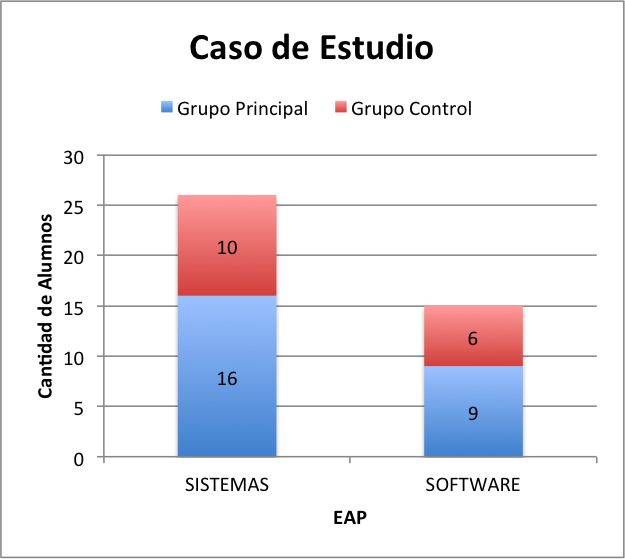
\includegraphics[scale=0.6]{figuras/chapter05/poblacion}}
\end{figure}

En este caso de estudio se formarán 3 grupos expertos los cuales desarrollarán problemas de estructuras selectivas y repetitivas(\texttt{if - for - while}). De esa forma, cuando se llegue a la reunión jigsaw, los grupos jigsaw contarán con expertos en problemas sobre los 3 tipos de estructuras.

\section{Definición de temas para el caso de estudio}
\subsection{Estructuras selectivas y repetitivas}
El tema ha desarrollarse en este caso de estudio es el de las estructuras selectivas \texttt{if - else} y las estructuras repetitivas \texttt{for, vhile}.\\

La sentencia \texttt{if} es referida comunmente para sentencias de decisión. Cada vez que se usan este tipo de sentencias en un programa, se le pide al programa evaluar una expresión para determinar que acción debe tomar.\\

La sintaxis de la sentencia \texttt{if} en java y/o c++ es la siguiente:\\

\begin{lstlisting}
if (booleanExpression) {
	...
}else{
	...
}
\end{lstlisting}


Las iteraciones permiten repetir bloques de código tantas veces como se establezca en la condición de la estructura repetitiva \texttt{for} o \texttt{while}. El \texttt{while} es bueno cuando se tienen escenarios en los cuales no se conoce de antemano la cantidad de veces que un bloque o una sentencia debe repetirse, pero se requiere repetirlas mientras la condición del \texttt{while} sea verdadera.\\

\begin{lstlisting}
while (expression){
	//bloque de codigo
}
\end{lstlisting}

La estructura \texttt{for} es especialmente usada cuando se conoce de antemano cuántas veces se necesita ejecutar las instrucciones que van dentro del bloque \texttt{for}. El \texttt{for} tiene 3 partes :

\begin{itemize}
	\item Declaración e inicialización de variables.
	\item La expresión a ser evaluada como verdadero o falso.
	\item La expresión de iteración.
\end{itemize}

Estas 3 partes son separadas por un punto y coma. La sintaxis de un \texttt{for} tanto para Java y C++ es la siguiente:

\begin{lstlisting}
for (/*Inicializacion*/ ; /*Condicion*/ ; /* Iteracion */) {
	/* body */
}

for (int i = 0; i < 10; i++) {
	/* body */
}
\end{lstlisting}


\subsection{Problemas}
\label{sec:problemas}
Para este caso de estudio se plante la resolución de los siguientes problemas de estructuras selectivas y estructuras repetitivas los cuales podrán ser desarrollados usando cualquiera de los 3 lenguajes que el Sistema Jigsaw Coding permite usar (Java, C++ o Python)\\

Para la fase de reunión de expertos y reunión jigsaw se usarán los siguientes problemas:

\begin{enumerate}
	\item \textbf{Par o impar}. Elaborar un programa que lea un entero y determine si es un número par o impar.
	\item \textbf{Múltiplos de 7}. Elaborar un programa que imprima los primeros 10 números múltiplos de 7 usando la estructura repetitiva \texttt{for}.
	\item \textbf{Números descendentes}. Elaborar un programa que imprima de forma descendente los primeros 20 numeros pares usando una estructura repetitiva \texttt{while}.
\end{enumerate}

Finalmente, para la fase de evaluación se combinará problemas de estructuras selectivas y repetitivas:

\begin{enumerate}
 	\item \textbf{Número mayor}. Elaborar un programa que lea dos números enteros y muestre el número mayor.
 	\item \textbf{n múltiplos de a}. Elaborar un programa que muestre los n primeros múltiplos de a, donde n y a son ingresados por teclado.
 	\item \textbf{De número a texto}. Elaborar un programa que lea un número del 1 al 5 y lo muestre de forma escrita. Ejemplo 1 $\longrightarrow$ uno. Si es un número distinto a 1,2,3,4 o 5 que muestre el mensaje: Número equivocado.
 	\item \textbf{Asteriscos}. Elaborar un programa que imprima la siguiente serie de asteriscos: \newline 	
 		\hbox{*} \newline
 		\hbox{**} \newline
 		\hbox{***} \newline
 		\hbox{****} \newline
 		\hbox{*****} 	
\end{enumerate}

\section{Aplicación del Sistema Jigsaw Coding al caso de estudio}
En esta sección se describe la secuencia de pasos que se realizaron para aplicar el sistema jigsaw coding al caso estudio descrito anteriormente.

\subsection{Creación de la sesión jigsaw}

\paragraph{Paso 1}
Se realizó la creación de los problemas que serían parte de la sesión de aprendizaje jigsaw. Todos los problemas descritos en el apartado anterior fueron ingresados al Sistema Jigsaw Coding, tal y como se puede apreciar en la \autoref{fig:c5_creacion_problemas}.

\begin{figure}
\centering
\caption{Creación de problemas.}
\label{fig:c5_creacion_problemas}
\fbox{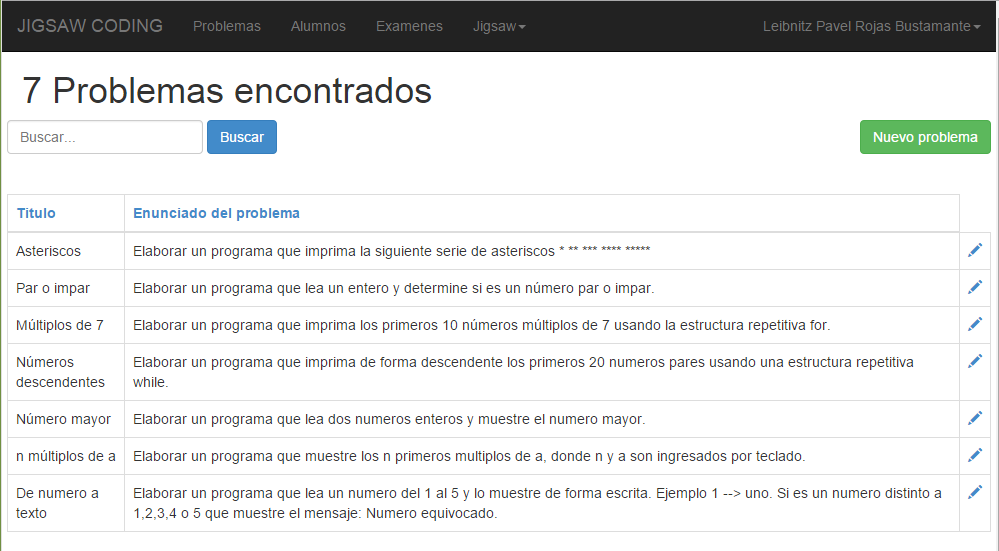
\includegraphics[scale=0.5]{figuras/chapter05/creacion_problemas}}
\end{figure}

\paragraph{Paso 2}
Tal como se muestra en la \autoref{fig:c5_creacion_alumnos}, se crearon las respectivas cuentas de usuario para los estudiantes que formarían parte de la sesión jigsaw. A cada de uno de ellos se les solicitó sus datos personales como DNI, Apellidos, Nombres y Correo electrónico para poder registrarlos en el Sistema. Luego de ello, se envió a cada estudiante sus respectivas credenciales para acceder al sistema.

\begin{figure}
	\centering
	\caption{Creación de cuentas de usuario para alumnos.}
	\label{fig:c5_creacion_alumnos}
	\fbox{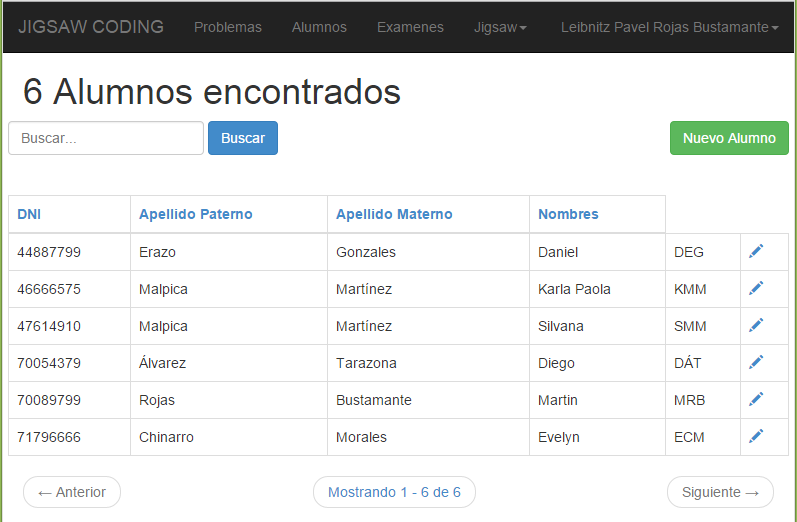
\includegraphics[scale=0.5]{figuras/chapter05/creacion_alumnos}}
\end{figure}

\paragraph{Paso 3}
Ya con los problema y alumnos registrados correctamente en el sistema, lo siguiente fue elaborar el examen que debía incluirse posteriormente en la fase de evaluación de la sesión jigsaw. Para esto, se creó un Nuevo Examen en el sistema y se agregaron los siguientes problemas: \emph{Número mayor, n múltiplos de a, De número a texto y Asteriscos}. A cada uno de ellos se les asignó un valor de 5 puntos para tener un total de 20 puntos para el examen. Ver \autoref{fig:c5_creacion_examen}.

\begin{figure}
	\centering
	\caption{Creación del examen para la fase de evaluación.}
	\label{fig:c5_creacion_examen}
	\fbox{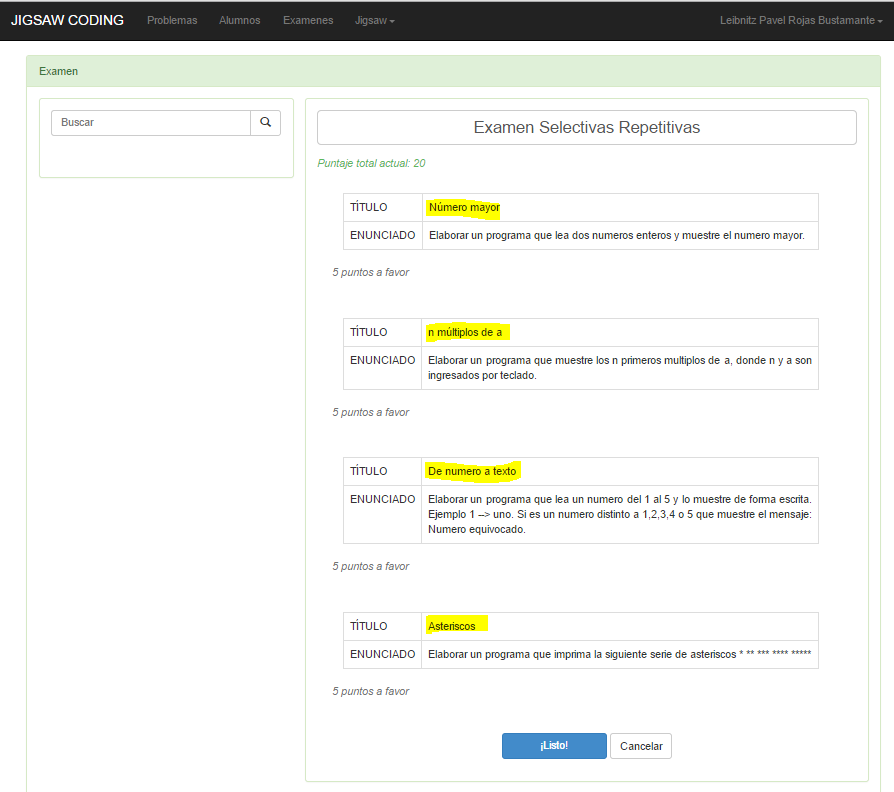
\includegraphics[scale=0.4]{figuras/chapter05/creacion_examen}}
\end{figure}

\paragraph{Paso 4}
En la \autoref{fig:c5_creacion_sesion_jigsaw} se puede observar que en este paso se realizó la creación de la sesión jigsaw a la cual se asignó que debería formar 3 grupos expertos y que el tema sería: \texttt{Estructuras Selectivas y Repetitivas.} 

\begin{figure}
	\centering
	\caption{Creación de la sesión jigsaw.}
	\label{fig:c5_creacion_sesion_jigsaw}
	\fbox{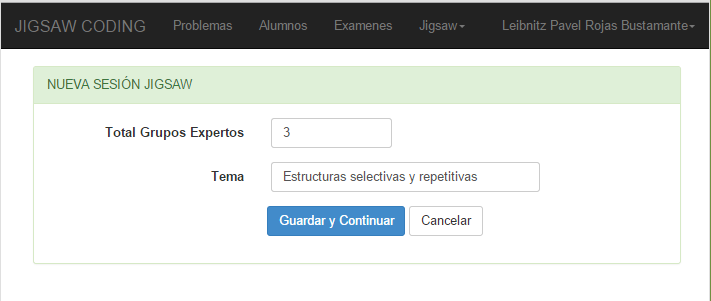
\includegraphics[scale=0.6]{figuras/chapter05/creacion_sesion_jigsaw}}
\end{figure}

\paragraph{Paso 5}
Este paso consistió en asignar qué alumnos participarían de la sesión jigsaw. Ver \autoref{fig:c5_asignacion_alumnos}.

\begin{figure}
	\centering
	\caption{Asignación de alumnos a la sesión jigsaw.}
	\label{fig:c5_asignacion_alumnos}
	\fbox{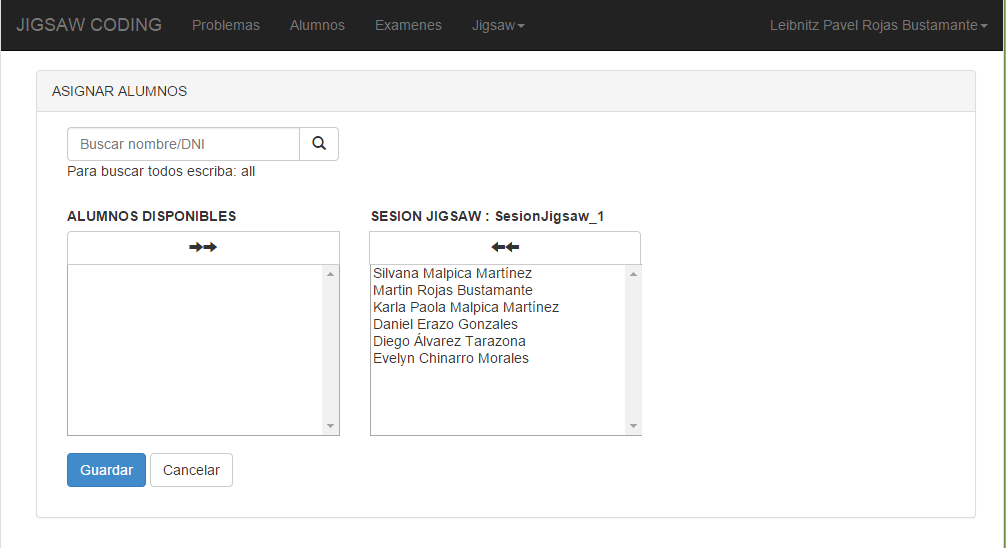
\includegraphics[scale=0.4]{figuras/chapter05/asignacion_alumnos}}
\end{figure}

\paragraph{Paso 6}
Despúes de asignar los alumnos a la sesión jigsaw, se presionó el botón Generar Grupos y el sistema generó aleatoriamente los 3 grupos expertos y los 2 grupos jigsaw con los cuales se trabajaría la sesión jigsaw. Los grupos generados por el sistema se muestran en la \autoref{fig:c5_grupos_generados}.

\begin{figure}
	\centering
	\caption{Grupos generados por el Sistema Jigsaw Coding.}
	\label{fig:c5_grupos_generados}
	\fbox{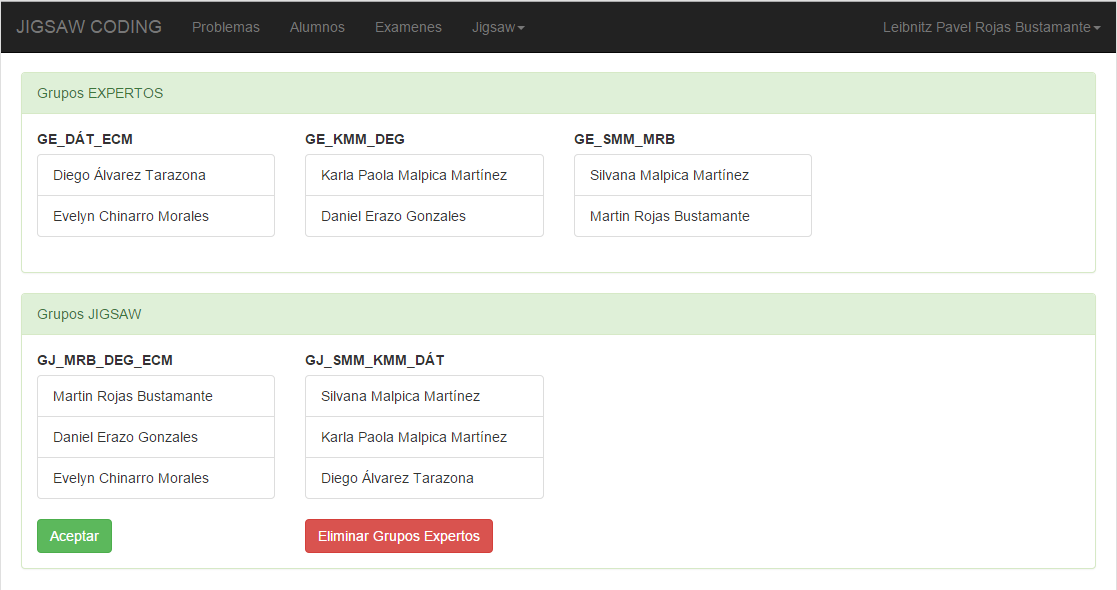
\includegraphics[scale=0.35]{figuras/chapter05/grupos_generados}}
\end{figure}

\paragraph{Paso 7}
Luego de tener definidos los grupos de la sesión jigsaw, se asignó el examen que sería utilizado y, posteriormente, se definió qué problema debería resolver cada uno de los grupos expertos, tal como se muestra en la \autoref{fig:c5_asignacion_problemas} y el la \autoref{tab:c5_asignacion_problemas}.

\begin{figure}[h!]
	\centering
	\caption{Asignación de problemas a grupos expertos}
	\label{fig:c5_asignacion_problemas}
	\fbox{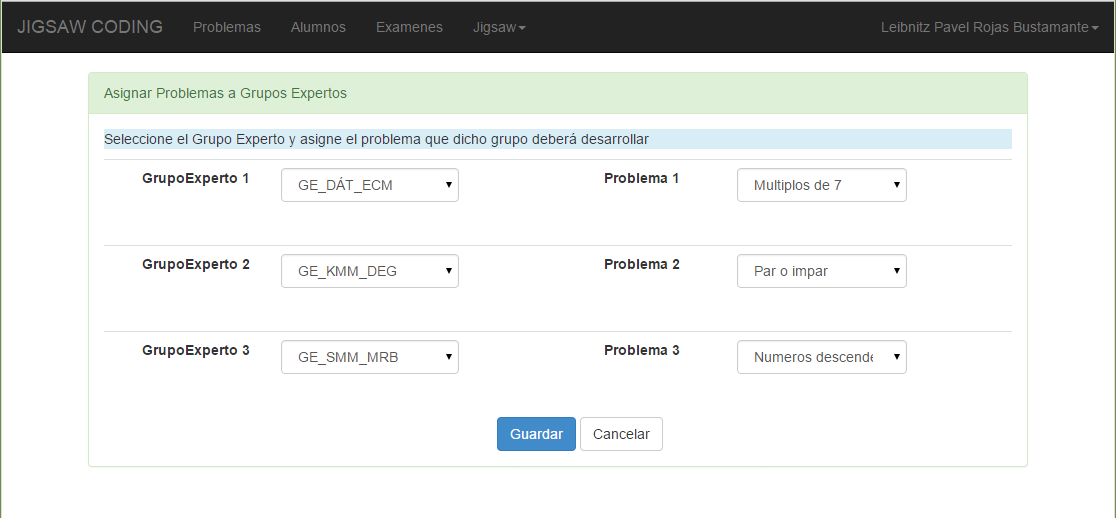
\includegraphics[scale=0.4]{figuras/chapter05/asignacion_problemas}}
\end{figure}

\begin{longtable}{ll}
	\caption{Asignación de problemas a grupos expertos}	
	\label{tab:c5_asignacion_problemas}\\
	\toprule[0.8mm]
	GRUPO EXPERTO & PROBLEMA \\
	\midrule
	GE\_DÁT\_ECM & Múltiplos de 7\\
	GE\_KMM\_DEG & Par o impar\\
	GE\_SMM\_MRB & Números descendentes\\
	\bottomrule[0.8mm]	
\end{longtable}

\paragraph{Paso 8}
Finalmente, se definió el horario para la reunión de expertos (\autoref{fig:c5_horario_reunion_expertos}), reunión jigsaw (\autoref{fig:c5_horario_reunion_jigsaw}) y evaluación (\autoref{fig:c5_horario_examen}). Los valores que se asignaron a estos horarios se encuentran en la \autoref{tab:c5_horarios_fases_jigsaw}.

\begin{longtable}{|l|l|l|}
	\caption{Horarios de las fases de la sesión jigsaw}	
	\label{tab:c5_horarios_fases_jigsaw}\\
	\toprule[0.8mm]
	REUNIÓN DE EXPERTOS & REUNIÓN JIGSAW & EXAMEN \\
	\midrule
	Fecha: 30-nov-2014 & Fecha: 30-nov-2014 & Fecha: 30-nov-2014\\
	Hora: 10:00 PM & Hora: 10:15 PM & Hora: 10:30 PM\\
	Duración: 10 minutos & Duración: 15 minutos & Duración: 30 minutos\\
	\bottomrule[0.8mm]

\end{longtable}
 
\begin{figure}
	\centering
	\caption{Horario reunión de expertos}
	\label{fig:c5_horario_reunion_expertos}
	\fbox{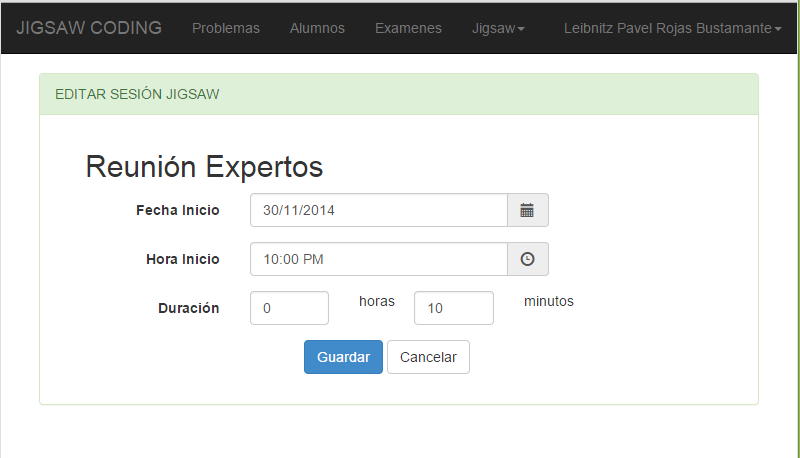
\includegraphics[scale=0.45]{figuras/chapter05/horario_reunion_expertos}}
\end{figure}
\clearpage
\begin{figure}
	\centering
	\caption{Horario reunión jigsaw}
	\label{fig:c5_horario_reunion_jigsaw}
	\fbox{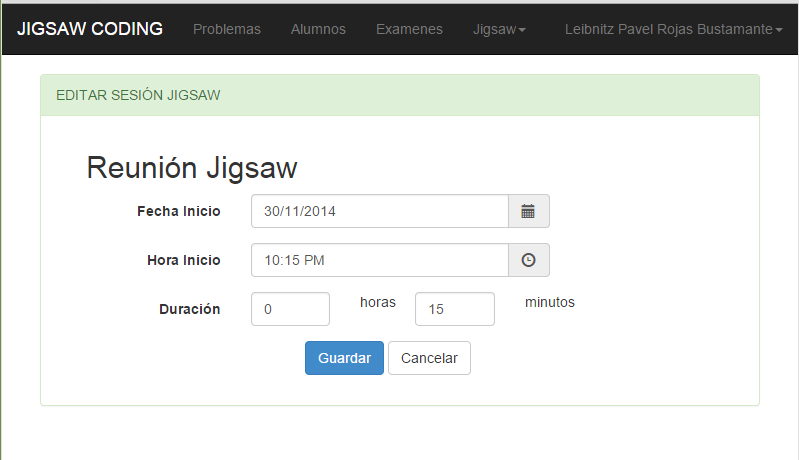
\includegraphics[scale=0.45]{figuras/chapter05/horario_reunion_jigsaw}}
\end{figure}

\begin{figure}
	\centering
	\caption{Horario del examen}
	\label{fig:c5_horario_examen}
	\fbox{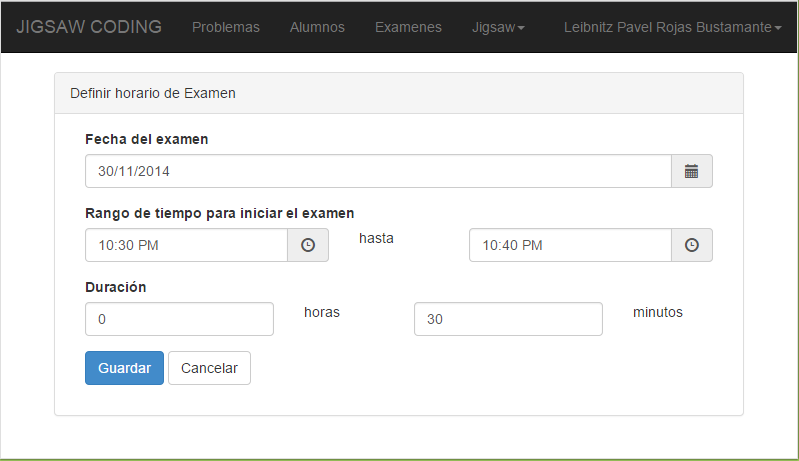
\includegraphics[scale=0.45]{figuras/chapter05/horario_examen}}
\end{figure}

\subsection{Desarrollo de la fase de Expertos}
La fase de reunión de expertos empezó a las 10:00 PM del 30 de noviembre del 2014, tal y como fue programado en el Sistema Jigsaw Coding.\\

Cada participante accedió al sistema y se unió a su respectivo grupo experto para dar solución al problema que tenían asignado. Para esta tarea cada grupo experto dispuso de un tiempo de 10 minutos, luego del cual, el sistema automáticamente cerró el panel de reunión de expertos.\\

\begin{figure}
	\centering
	\caption[Reunión de Expertos - Evelyn Chinarro]{Pantalla de la participante Evelyn Chinarro durante la reunión de expertos.}
	\label{fig:c5_reunion_expertos_evy}
	\fbox{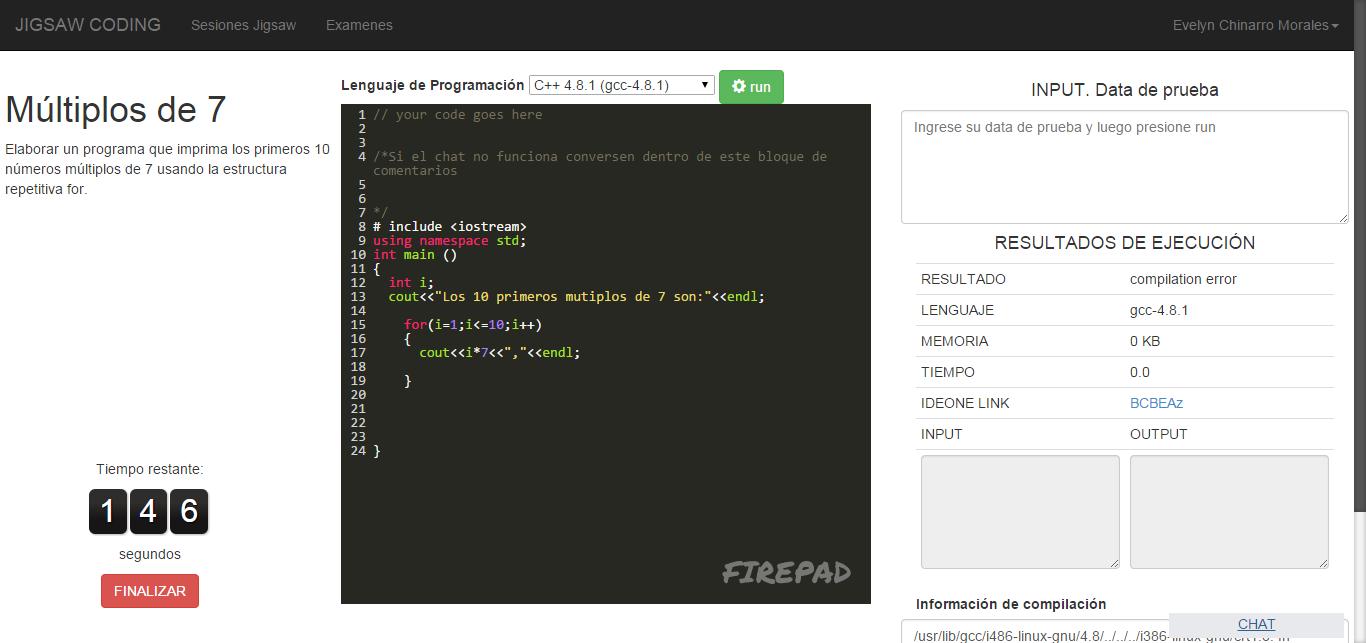
\includegraphics[scale=0.4]{figuras/chapter05/reunion_expertos/evy}}
\end{figure}

En la \autoref{fig:c5_reunion_expertos_evy}, la participante Evelyn desarrolló de manera colaborativa el problema \textbf{Múltiplos de 7} junto con Diego Álvarez, el segundo miembro del grupo experto \textbf{GE\_DÁT\_ECM}. Ambos usaron el lenguaje de programación C++.\\

\begin{figure}
	\centering
	\caption[Reunión de Expertos - Martin Rojas]{Pantalla del participante Martin Rojas durante la reunión de expertos.}
	\label{fig:c5_reunion_expertos_martin}
	\fbox{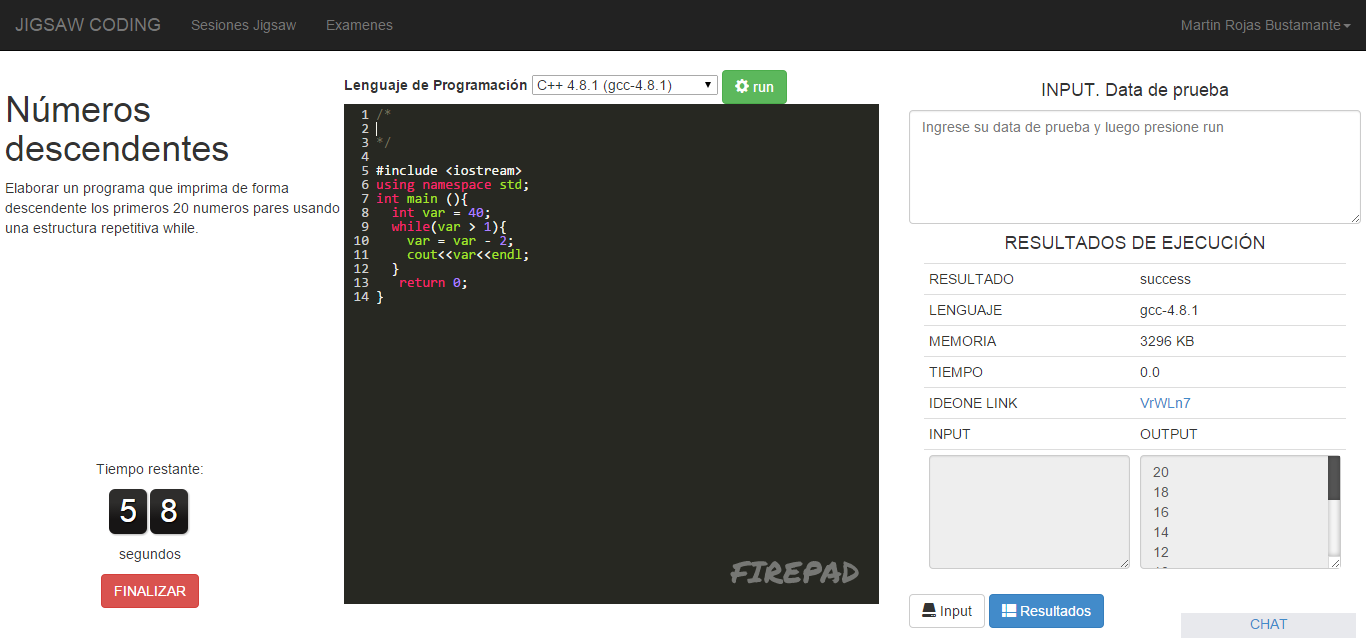
\includegraphics[scale=0.4]{figuras/chapter05/reunion_expertos/martin}}
\end{figure}

Por otro lado, en la \autoref{fig:c5_reunion_expertos_martin} se tiene al participante Martin Rojas, miembro del grupo experto \textbf{GE\_SMM\_MRB}, desarrollando en C++ el problema \textbf{Números descendentes}.\\

Así mismo, el participante Daniel Erazo, del grupo experto \textbf{GE\_KMM\_DEG},  desarrolló junto a Karla Malpica el problema \textbf{Par o impar}. Este grupo optó por usar el lenguaje de programación Java. Ver \autoref{fig:c5_reunion_expertos_daniel}.

\begin{figure}
	\centering
	\caption[Reunión de Expertos - Daniel Erazo]{Pantalla del participante Daniel Erazo durante la reunión de expertos.}
	\label{fig:c5_reunion_expertos_daniel}
	\fbox{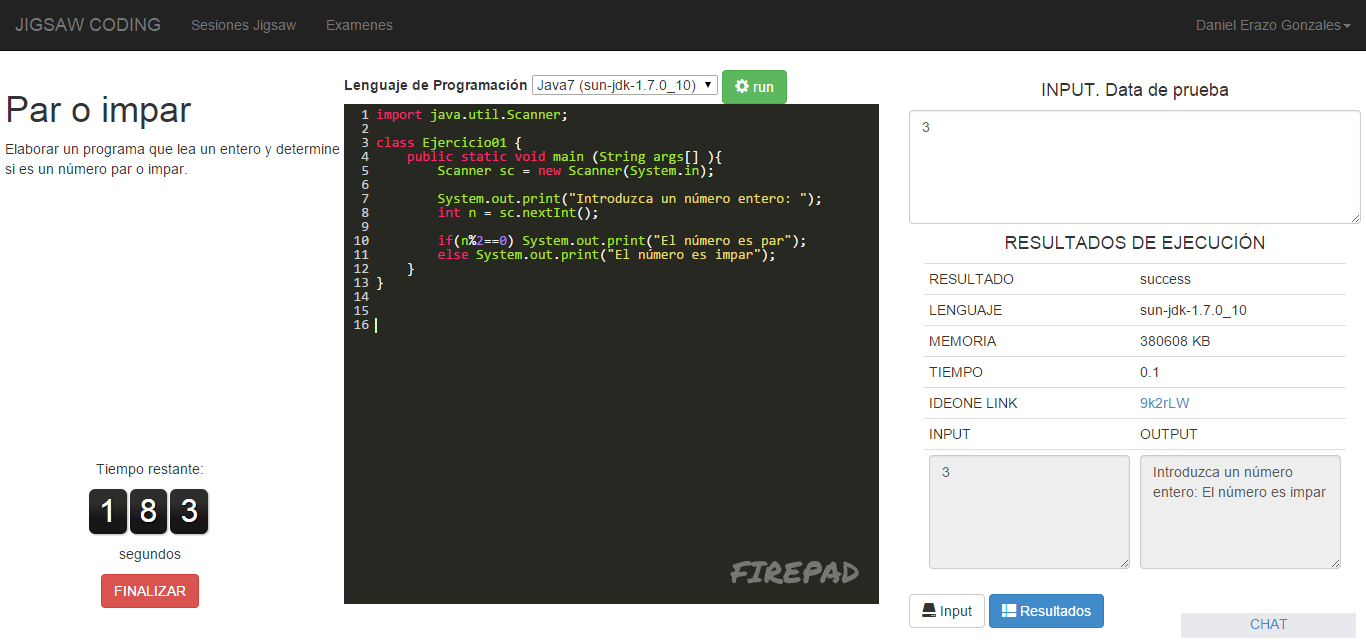
\includegraphics[scale=0.4]{figuras/chapter05/reunion_expertos/daniel}}
\end{figure}

\subsection{Desarrollo de la fase Jigsaw}
La fase de reunión jigsaw empezó a las 10:15 PM del 30 de noviembre del 2014, y esta duró 15 minutos. En ese tiempo, en cada grupo jigsaw se resolvieron los 3 problemas que cada grupo experto hizo en la fase anterior. Cabe recalcar que en esta fase, cada grupo contaba con un miembro experto en la resolución de un determinado problema; esto es, en cada grupo jigsaw había un alumno experto en una de las 3 estructuras de programación planteadas para esta sesión jigsaw (if - for - while).\\

La \autoref{fig:c5_reunion_jigsaw_silvana} muestra el momento en que el grupo jigsaw conformado por Silvana, Karla y Diego (GJ\_SMM\_KMM\_DÁT) resolvía los problemas \emph{Par o impar, Múltiplos de 7 y Números descendentes}.

\begin{figure}
	\centering
	\caption[Reunión Jigsaw - Silvana Malpica]{Pantalla de la participante Silvana Malpica durante la reunión jigsaw.}
	\label{fig:c5_reunion_jigsaw_silvana}
	\fbox{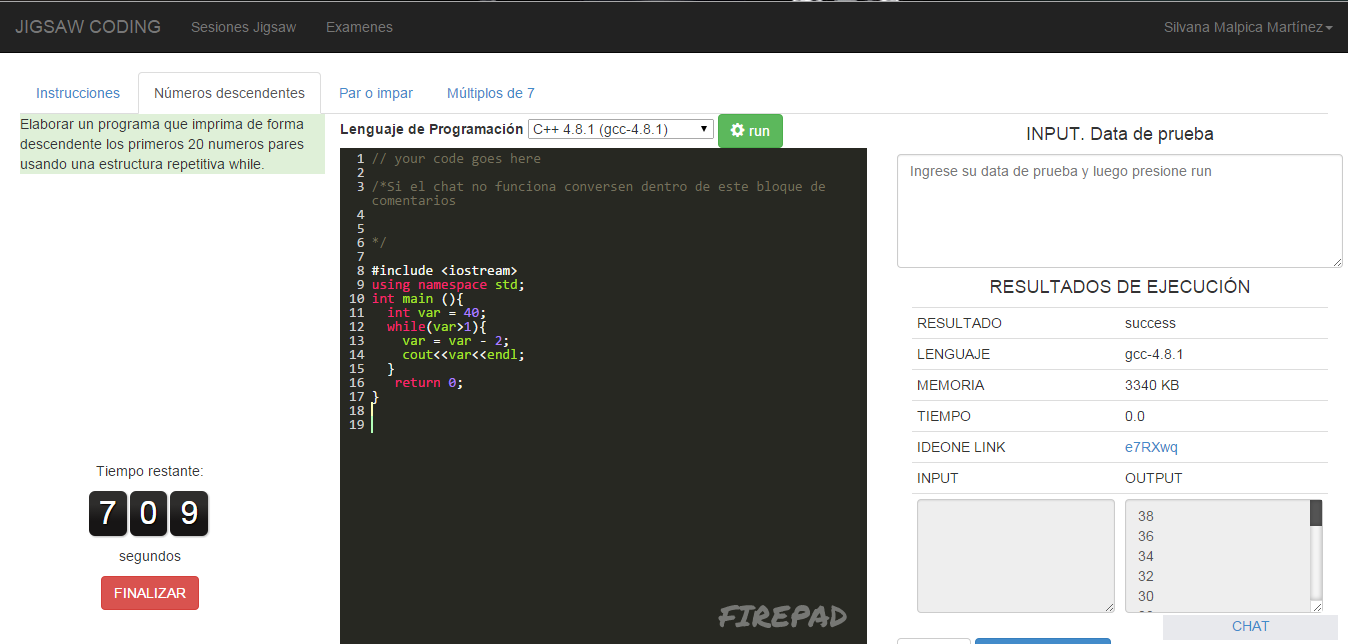
\includegraphics[scale=0.4]{figuras/chapter05/reunion_jigsaw/silvana}}
\end{figure}

\subsection{Desarrollo de la fase de Evaluación}
La última fase de la sesión jigsaw trata sobre la aplicación de un examen a los participantes de la dinámica. Este examen fue resuelto por cada alumno de manera individual y se plantearon 4 problemas, los mismo que debieron ser solucionados en un lapso de 30 minutos. El inicio del examen se dio a las 10:30 PM del 30 de noviembre del 2014. Cada alumno fue libre de escoger el lenguaje de programación de su preferencia para la resolución de cada problema del examen.\\

En la \autoref{fig:c5_evaluacion_diego} se muestra una de las soluciones del participante Diego Álvarez durante la fase de evaluación. Él utilizó para el desarrollo del problema \textbf{De número a texto} el lenguaje de programación C++.\\

\begin{figure}
	\centering
	\caption[Evaluación - Diego Álvarez]{Pantalla del participante Diego Álvarez durante la fase de evaluación.}
	\label{fig:c5_evaluacion_diego}
	\fbox{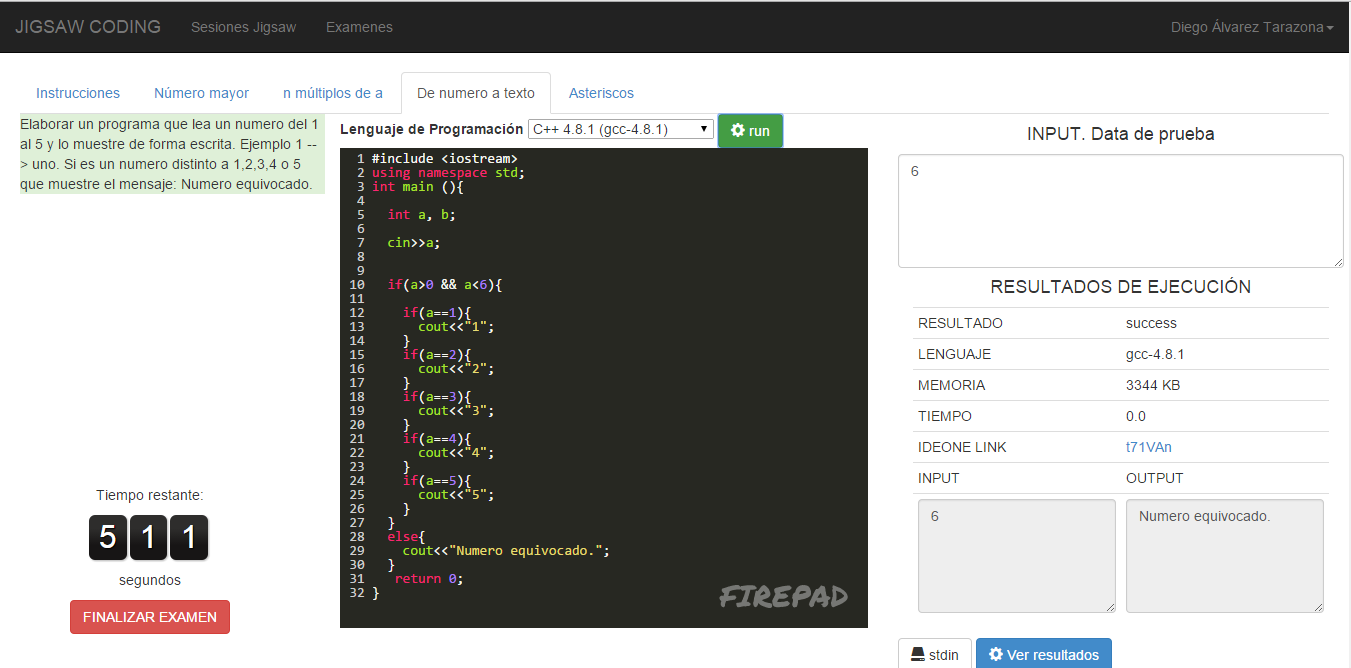
\includegraphics[scale=0.4]{figuras/chapter05/evaluacion/diego}}
\end{figure}

Finalmente, cuando se cumplió el tiempo establecido para el desarrollo del examen, se guardaron las respuestas de los alumnos y se dio por culminada la sesión jigsaw para el aprendizaje de estructuras repetitivas y selectivas.